
% This LaTeX was auto-generated from MATLAB code.
% To make changes, update the MATLAB code and republish this document.

\documentclass{article}
\usepackage{graphicx}
\usepackage{color}

\sloppy
\definecolor{lightgray}{gray}{0.5}
\setlength{\parindent}{0pt}

\begin{document}

    
    
\section*{Math 315 Lab 7}

\begin{par}
The following lab compares the convergence rates of Gauss and Clenshaw-Curtis quadrature.
\end{par} \vspace{1em}

\subsection*{Contents}

\begin{itemize}
\setlength{\itemsep}{-1ex}
   \item Gauss Quadrature Code
   \item Clenshaw-Curtis Quadrature Code
   \item x\^{}20
   \item e\^{}x
   \item e\^{}(-x\^{}2)
   \item 1/(1+16x\^{}2)
   \item e\^{}(-x\^{}-2)
   \item \ensuremath{|} x \ensuremath{|}\^{}3
   \item Convergence of Errors
   \item Degree of Precision
\end{itemize}


\subsection*{Gauss Quadrature Code}

\begin{par}
The following code approximates the integral of f on the interval -1 to 1 using Gauss Quadrature.
\end{par} \vspace{1em}
\begin{verbatim}
disp(fileread("gauss.m"));
\end{verbatim}

        \color{lightgray} \begin{verbatim}function I = gauss(f, n)
    beta = .5./sqrt(1-(2*(1:n)).^(-2)); 
    T = diag(beta,1) + diag(beta,-1);
    [V,D] = eig(T);
    x = diag(D); [x,i] = sort(x);
    w = 2*V(1,i).^2;
    I = w*feval(f,x);
\end{verbatim} \color{black}
    

\subsection*{Clenshaw-Curtis Quadrature Code}

\begin{par}
The following code approximates the integral of f on the interval -1 to 1 using Clenshaw-Curtis Quadrature.
\end{par} \vspace{1em}
\begin{verbatim}
disp(fileread("clenshawcurtis.m"));
\end{verbatim}

        \color{lightgray} \begin{verbatim}function I = clenshaw_curtis(f,n)
    x = cos(pi*(0:n)'/n);
    fx = feval(f,x)/(2*n);
    g = real(fft(fx([1:n+1 n:-1:2])));
    a = [g(1); g(2:n)+g(2*n:-1:n+2); g(n+1)];
    w = 0*a'; w(1:2:end) = 2./(1-(0:2:n).^2);
    I = w*a;
\end{verbatim} \color{black}
    

\subsection*{x\^{}20}

\begin{par}
Using both Gauss and Clenshaw-Curtis Quadrature, I will approximate the integral of x\^{}20 on the interval -1 to 1.
\end{par} \vspace{1em}
\begin{verbatim}
f = @(x) x.^20;
true_I = 2/21;
N = 30;
gauss_I_1 = zeros(1, N);
clenshawcurtis_I_1 = zeros(1, N);

for n = 1:N
    gauss_I_1(n) = gauss(f, n);
    clenshawcurtis_I_1(n) = clenshawcurtis(f, n);
end

gauss_err_1 = abs(gauss_I_1 - true_I);
clenshawcurtis_err_1 = abs(clenshawcurtis_I_1 - true_I);
\end{verbatim}


\subsection*{e\^{}x}

\begin{par}
Using both Gauss and Clenshaw-Curtis Quadrature, I will approximate the integral of e\^{}x on the interval -1 to 1.
\end{par} \vspace{1em}
\begin{verbatim}
f = @(x) exp(x);
true_I = exp(1) - 1/exp(1);
N = 30;
gauss_I_2 = zeros(1, N);
clenshawcurtis_I_2 = zeros(1, N);

for n = 1:N
    gauss_I_2(n) = gauss(f, n);
    clenshawcurtis_I_2(n) = clenshawcurtis(f, n);
end

gauss_err_2 = abs(gauss_I_2 - true_I);
clenshawcurtis_err_2 = abs(clenshawcurtis_I_2 - true_I);
\end{verbatim}


\subsection*{e\^{}(-x\^{}2)}

\begin{par}
Using both Gauss and Clenshaw-Curtis Quadrature, I will approximate the integral of e\^{}(-x\^{}2) on the interval -1 to 1.
\end{par} \vspace{1em}
\begin{verbatim}
f = @(x) exp(-x.^2);
true_I = integral(f, -1, 1);
N = 30;
gauss_I_3 = zeros(1, N);
clenshawcurtis_I_3 = zeros(1, N);

for n = 1:N
    gauss_I_3(n) = gauss(f, n);
    clenshawcurtis_I_3(n) = clenshawcurtis(f, n);
end

gauss_err_3 = abs(gauss_I_3 - true_I);
clenshawcurtis_err_3 = abs(clenshawcurtis_I_3 - true_I);
\end{verbatim}


\subsection*{1/(1+16x\^{}2)}

\begin{par}
Using both Gauss and Clenshaw-Curtis Quadrature, I will approximate the integral of 1/(1+16x\^{}2) on the interval -1 to 1.
\end{par} \vspace{1em}
\begin{verbatim}
f = @(x) 1./(1+16*x.^2);
true_I = 0.5*atan(4);
N = 30;
gauss_I_4 = zeros(1, N);
clenshawcurtis_I_4 = zeros(1, N);

for n = 1:N
    gauss_I_4(n) = gauss(f, n);
    clenshawcurtis_I_4(n) = clenshawcurtis(f, n);
end

gauss_err_4 = abs(gauss_I_4 - true_I);
clenshawcurtis_err_4 = abs(clenshawcurtis_I_4 - true_I);
\end{verbatim}


\subsection*{e\^{}(-x\^{}-2)}

\begin{par}
Using both Gauss and Clenshaw-Curtis Quadrature, I will approximate the integral of e\^{}(-x\^{}-2) on the interval -1 to 1.
\end{par} \vspace{1em}
\begin{verbatim}
f = @(x) exp(-x.^-2);
true_I = integral(f, -1, 1);
N = 30;
gauss_I_5 = zeros(1, N);
clenshawcurtis_I_5 = zeros(1, N);

for n = 1:N
    gauss_I_5(n) = gauss(f, n);
    clenshawcurtis_I_5(n) = clenshawcurtis(f, n);
end

gauss_err_5 = abs(gauss_I_5 - true_I);
clenshawcurtis_err_5 = abs(clenshawcurtis_I_5 - true_I);
\end{verbatim}


\subsection*{\ensuremath{|} x \ensuremath{|}\^{}3}

\begin{par}
Using both Gauss and Clenshaw-Curtis Quadrature, I will approximate the integral of \texttt{x}\^{}3 on the interval -1 to 1.
\end{par} \vspace{1em}
\begin{verbatim}
f = @(x) abs(x).^3;
true_I = 0.5;
N = 30;
gauss_I_6 = zeros(1, N);
clenshawcurtis_I_6 = zeros(1, N);

for n = 1:N
    gauss_I_6(n) = gauss(f, n);
    clenshawcurtis_I_6(n) = clenshawcurtis(f, n);
end

gauss_err_6 = abs(gauss_I_6 - true_I);
clenshawcurtis_err_6 = abs(clenshawcurtis_I_6 - true_I);
\end{verbatim}


\subsection*{Convergence of Errors}

\begin{par}
The convergence of errors for the integral approximations from Gauss and Clenshaw-Curtis Quadrature are plotted below for increasing n. The rate of convergence for the first 5 integrals are of order O(e\^{}-an) and the last integral is of order O(x\^{}-b). The exact coefficients a and b for the rate of convergence are shown below. This is because the first 5 functions are infinitely differentiable, whereas the last function is not infinitely differentiable.
\end{par} \vspace{1em}
\begin{verbatim}
close all;
figure1 = figure('Position', [100 100 800 1200]);
x = linspace(1, 30, 30);
gauss_x_fit = x(1:9);
gauss_fit = gauss_err_1(1:9);
gauss_p = polyfit(gauss_x_fit, log(gauss_fit), 1);
gauss_y_fit = exp(gauss_p(2)) * exp(gauss_x_fit .* gauss_p(1));
fprintf('Gauss Convergence for x^20: y = %g * e^%gx\n', exp(gauss_p(2)), ...
    gauss_p(1));
clenshawcurtis_x_fit = x(1:19);
clenshawcurtis_fit = clenshawcurtis_err_1(1:19);
clenshawcurtis_p = polyfit(clenshawcurtis_x_fit, log(clenshawcurtis_fit), 1);
clenshawcurtis_y_fit = exp(clenshawcurtis_p(2)) * exp(clenshawcurtis_x_fit ...
    .* clenshawcurtis_p(1));
fprintf('Clenshaw-Curtis Convergence for x^20: y = %g * e^%gx\n\n', ...
    exp(clenshawcurtis_p(2)), clenshawcurtis_p(1));
subplot(3,2,1);
semilogy(x, gauss_err_1, 'b--o', x, clenshawcurtis_err_1, 'r--o', ...
    gauss_x_fit, gauss_y_fit, 'k', clenshawcurtis_x_fit, ...
    clenshawcurtis_y_fit, 'm');
xlabel('n');
ylabel('abs err');
legend('Gauss', 'Clenshaw-Curtis', 'Gauss Convergence', ['Clenshaw-Curtis ' ...
    'Convergence'])
title('x^{20}')

gauss_x_fit = x(1:6);
gauss_fit = gauss_err_2(1:6);
gauss_p = polyfit(gauss_x_fit, log(gauss_fit), 1);
gauss_y_fit = exp(gauss_p(2)) * exp(gauss_x_fit .* gauss_p(1));
fprintf('Gauss Convergence for e^x: y = %g * e^%gx\n', exp(gauss_p(2)), ...
    gauss_p(1));
clenshawcurtis_x_fit = x(1:11);
clenshawcurtis_fit = clenshawcurtis_err_2(1:11);
clenshawcurtis_p = polyfit(clenshawcurtis_x_fit, log(clenshawcurtis_fit), 1);
clenshawcurtis_y_fit = exp(clenshawcurtis_p(2)) * exp(clenshawcurtis_x_fit ...
    .* clenshawcurtis_p(1));
fprintf('Clenshaw-Curtis Convergence for e^x: y = %g * e^%gx\n\n', ...
    exp(clenshawcurtis_p(2)), clenshawcurtis_p(1));
subplot(3,2,2);
semilogy(x, gauss_err_2, 'b--o', x, clenshawcurtis_err_2, 'r--o', ...
    gauss_x_fit, gauss_y_fit, 'k', clenshawcurtis_x_fit, clenshawcurtis_y_fit, 'm');
xlabel('n');
ylabel('abs err');
legend('Gauss', 'Clenshaw-Curtis', 'Gauss Convergence', ['Clenshaw-Curtis ' ...
    'Convergence'])
title('e^x')

gauss_x_fit = x(1:11);
gauss_fit = gauss_err_3(1:11);
gauss_p = polyfit(gauss_x_fit, log(gauss_fit), 1);
gauss_y_fit = exp(gauss_p(2)) * exp(gauss_x_fit .* gauss_p(1));
fprintf('Gauss Convergence for e^-x^2: y = %g * e^%gx\n', exp(gauss_p(2)), ...
    gauss_p(1));
clenshawcurtis_x_fit = x(1:19);
clenshawcurtis_fit = clenshawcurtis_err_3(1:19);
clenshawcurtis_p = polyfit(clenshawcurtis_x_fit, log(clenshawcurtis_fit), 1);
clenshawcurtis_y_fit = exp(clenshawcurtis_p(2)) * exp(clenshawcurtis_x_fit ...
    .* clenshawcurtis_p(1));
fprintf('Clenshaw-Curtis Convergence for e^-x^2: y = %g * e^%gx\n\n', ...
    exp(clenshawcurtis_p(2)), clenshawcurtis_p(1));
subplot(3,2,3);
semilogy(x, gauss_err_3, 'b--o', x, clenshawcurtis_err_3, 'r--o', ...
    gauss_x_fit, gauss_y_fit, 'k', clenshawcurtis_x_fit, clenshawcurtis_y_fit, 'm');
xlabel('n');
ylabel('abs err');
legend('Gauss', 'Clenshaw-Curtis', 'Gauss Convergence', ['Clenshaw-Curtis ' ...
    'Convergence'])
title('e^{-x^2}')

gauss_x_fit = x(1:30);
gauss_fit = gauss_err_4(1:30);
gauss_p = polyfit(gauss_x_fit, log(gauss_fit), 1);
gauss_y_fit = exp(gauss_p(2)) * exp(gauss_x_fit .* gauss_p(1));
fprintf('Gauss Convergence for 1/(1+16x^2): y = %g * e^%gx\n', ...
    exp(gauss_p(2)), gauss_p(1));
clenshawcurtis_x_fit = x(1:30);
clenshawcurtis_fit = clenshawcurtis_err_4(1:30);
clenshawcurtis_p = polyfit(clenshawcurtis_x_fit, log(clenshawcurtis_fit), 1);
clenshawcurtis_y_fit = exp(clenshawcurtis_p(2)) * exp(clenshawcurtis_x_fit ...
    .* clenshawcurtis_p(1));
fprintf('Clenshaw-Curtis Convergence for 1/(1+16x^2): y = %g * e^%gx\n\n', ...
    exp(clenshawcurtis_p(2)), clenshawcurtis_p(1));
subplot(3,2,4);
semilogy(x, gauss_err_4, 'b--o', x, clenshawcurtis_err_4, 'r--o', ...
    gauss_x_fit, gauss_y_fit, 'k', clenshawcurtis_x_fit, clenshawcurtis_y_fit, 'm');
xlabel('n');
ylabel('abs err');
legend('Gauss', 'Clenshaw-Curtis', 'Gauss Convergence', ['Clenshaw-Curtis ' ...
    'Convergence'])
title('1/(1+16x^2)')

gauss_x_fit = x(1:30);
gauss_fit = gauss_err_5(1:30);
gauss_p = polyfit(gauss_x_fit, log(gauss_fit), 1);
gauss_y_fit = exp(gauss_p(2)) * exp(gauss_x_fit .* gauss_p(1));
fprintf('Gauss Convergence for e^-x^-2: y = %g * e^%gx\n', exp(gauss_p(2)), ...
    gauss_p(1));
clenshawcurtis_x_fit = x(1:30);
clenshawcurtis_fit = clenshawcurtis_err_5(1:30);
clenshawcurtis_p = polyfit(clenshawcurtis_x_fit, log(clenshawcurtis_fit), 1);
clenshawcurtis_y_fit = exp(clenshawcurtis_p(2)) * exp(clenshawcurtis_x_fit ...
    .* clenshawcurtis_p(1));
fprintf('Clenshaw-Curtis Convergence for e^-x^-2: y = %g * e^%gx\n\n', ...
    exp(clenshawcurtis_p(2)), clenshawcurtis_p(1));
subplot(3,2,5);
semilogy(x, gauss_err_5, 'b--o', x, clenshawcurtis_err_5, 'r--o', ...
    gauss_x_fit, gauss_y_fit, 'k', clenshawcurtis_x_fit, clenshawcurtis_y_fit, 'm');
xlabel('n');
ylabel('abs err');
legend('Gauss', 'Clenshaw-Curtis', 'Gauss Convergence', ['Clenshaw-Curtis ' ...
    'Convergence'])
title('e^{-x^{-2}}')

gauss_x_fit = x(1:30);
gauss_fit = gauss_err_6(1:30);
gauss_p = polyfit(log(gauss_x_fit), log(gauss_fit), 1);
gauss_y_fit = exp(gauss_p(2)) * gauss_x_fit .^ gauss_p(1);
fprintf('Gauss Convergence for |x|^3: y = %g * x^%g\n', exp(gauss_p(2)), ...
    gauss_p(1));
clenshawcurtis_x_fit = x(1:30);
clenshawcurtis_fit = clenshawcurtis_err_6(1:30);
clenshawcurtis_p = polyfit(log(clenshawcurtis_x_fit), log(clenshawcurtis_fit), 1);
clenshawcurtis_y_fit = exp(clenshawcurtis_p(2)) * clenshawcurtis_x_fit .^ ...
    clenshawcurtis_p(1);
fprintf('Clenshaw-Curtis Convergence for |x|^3: y = %g * x^%g\n\n', ...
    exp(clenshawcurtis_p(2)), clenshawcurtis_p(1));
subplot(3,2,6);
semilogy(x, gauss_err_6, 'b--o', x, clenshawcurtis_err_6, 'r--o', ...
    gauss_x_fit, gauss_y_fit, 'k', clenshawcurtis_x_fit, clenshawcurtis_y_fit, 'm');
xlabel('n');
ylabel('abs err');
legend('Gauss', 'Clenshaw-Curtis', 'Gauss Convergence', ['Clenshaw-Curtis ' ...
    'Convergence'])
title('|x|^3')
\end{verbatim}

        \color{lightgray} \begin{verbatim}Gauss Convergence for x^20: y = 1.74504 * e^-1.2615x
Clenshaw-Curtis Convergence for x^20: y = 6.37064 * e^-1.07263x

Gauss Convergence for e^x: y = 5.29503 * e^-5.77107x
Clenshaw-Curtis Convergence for e^x: y = 21.7437 * e^-3.31919x

Gauss Convergence for e^-x^2: y = 4.33867 * e^-3.26612x
Clenshaw-Curtis Convergence for e^-x^2: y = 4.26161 * e^-1.9786x

Gauss Convergence for 1/(1+16x^2): y = 0.726662 * e^-0.493698x
Clenshaw-Curtis Convergence for 1/(1+16x^2): y = 1.4876 * e^-0.492467x

Gauss Convergence for e^-x^-2: y = 0.0200237 * e^-0.461993x
Clenshaw-Curtis Convergence for e^-x^-2: y = 0.0845879 * e^-0.487507x

Gauss Convergence for |x|^3: y = 0.191174 * x^-3.3939
Clenshaw-Curtis Convergence for |x|^3: y = 2.47692 * x^-4.15563

\end{verbatim} \color{black}
    
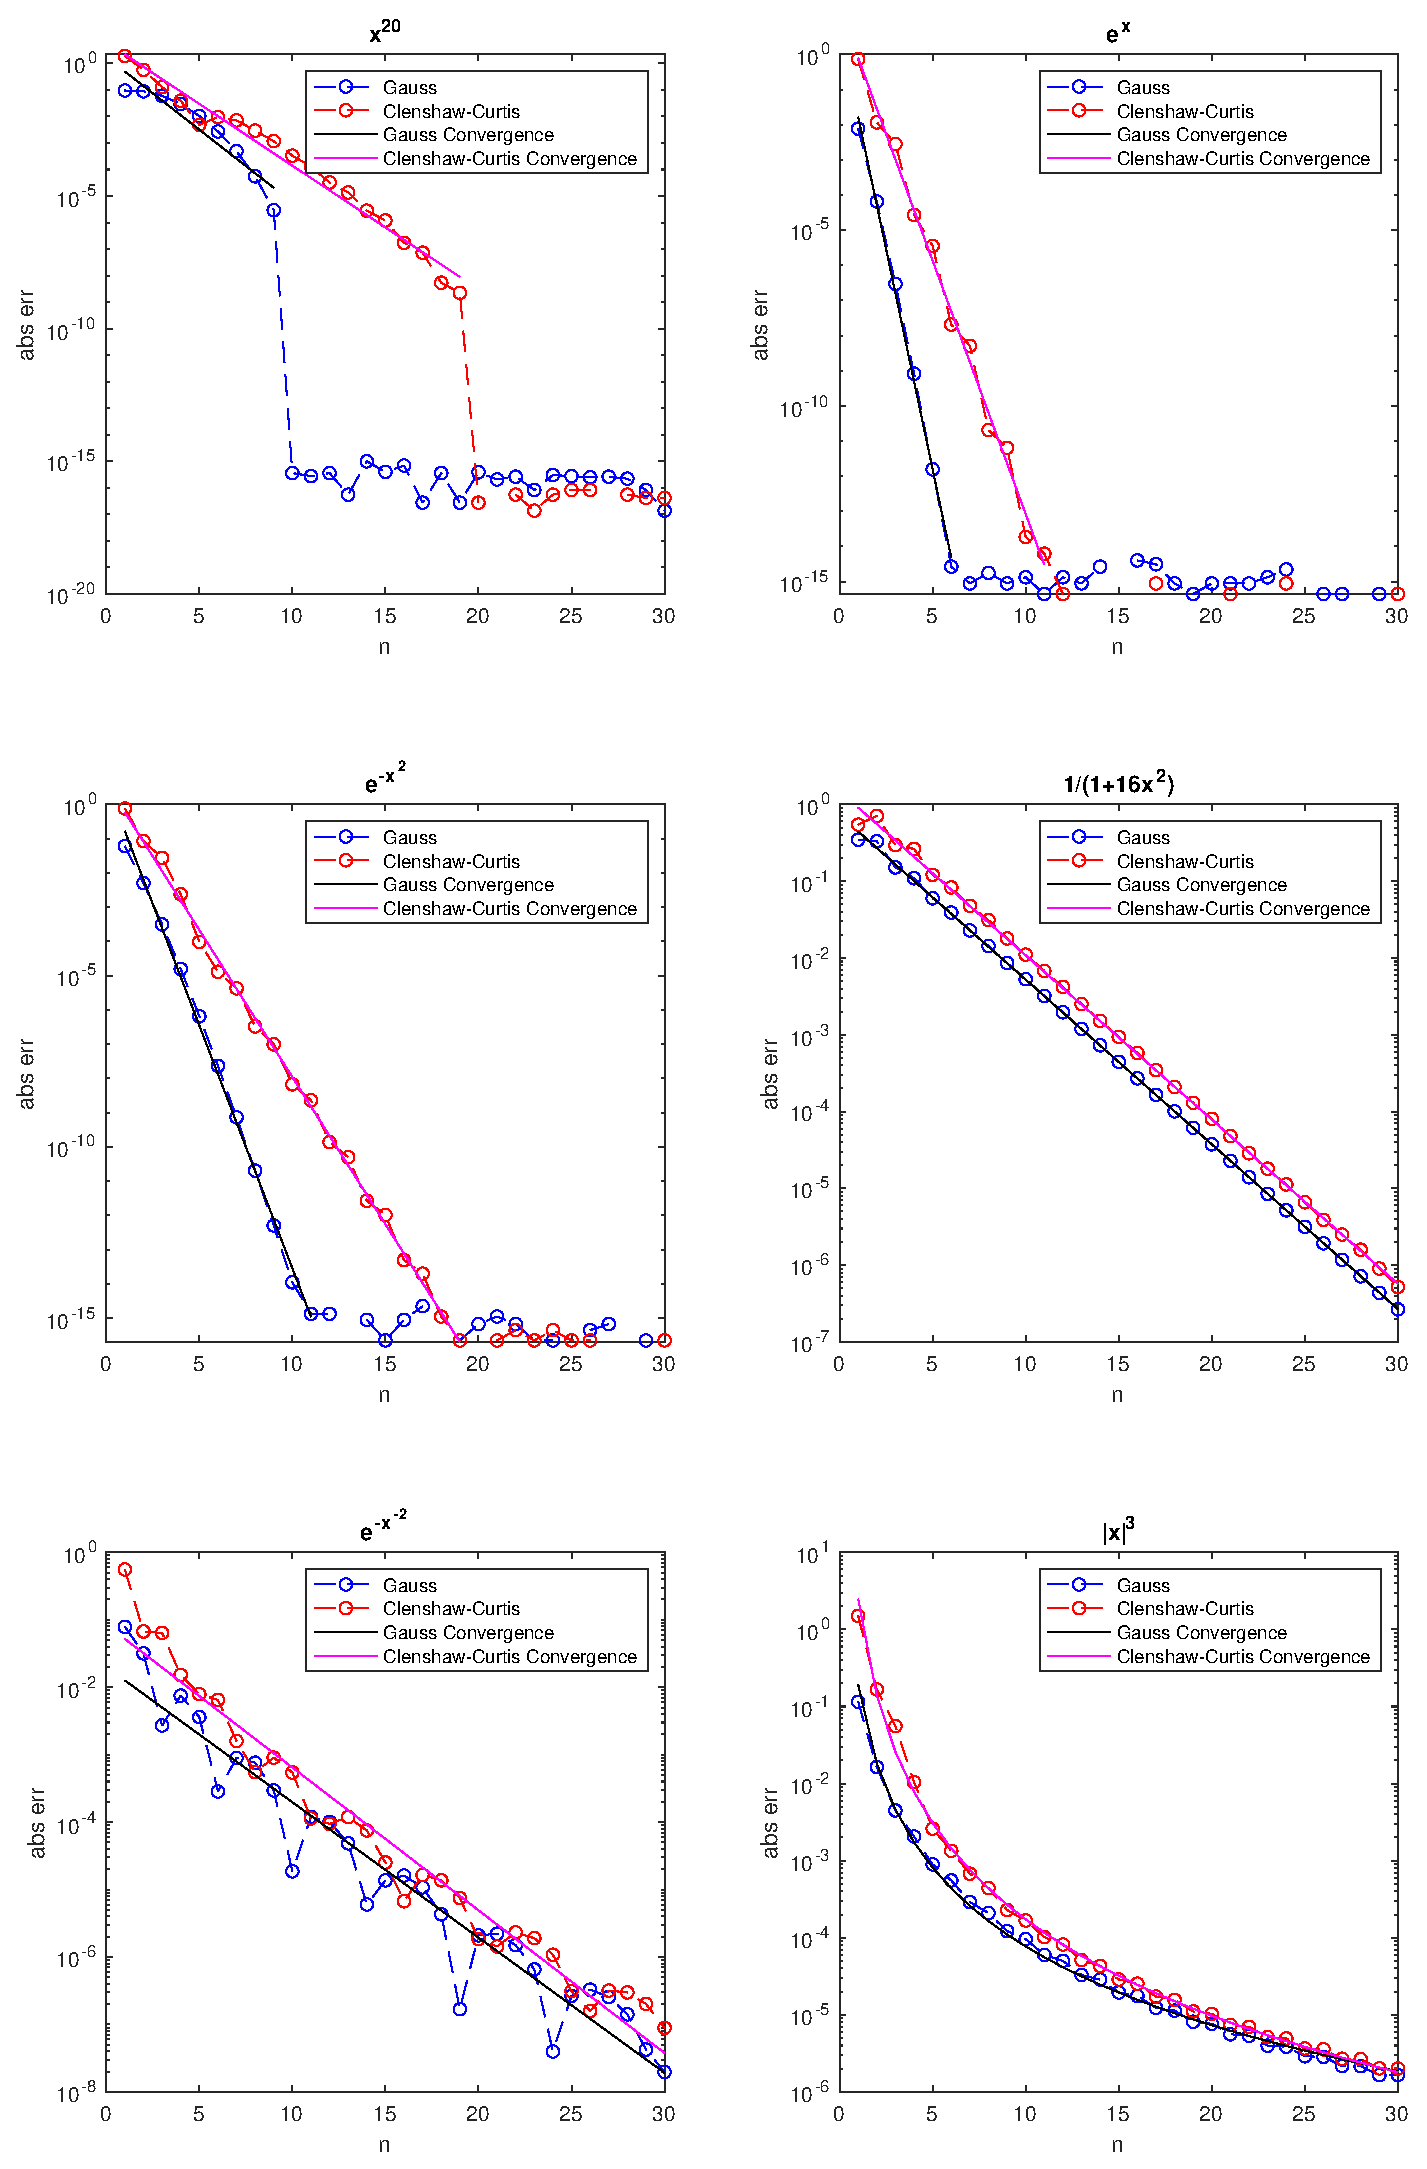
\includegraphics [width=4in]{Lab7_01.eps}


\subsection*{Degree of Precision}

\begin{par}
The degree of precision for Gauss Quadrature is 2N-1 and the degree of precision for Clenshaw-Curtis Quadrature is N, where N is the number of points. In the code, the n represents the degree of the underlying interpolant. Therefore the number of points N=n+1.
\end{par} \vspace{1em}
\begin{par}
The degree of precision for Gauss and Clenshaw-Curtis are shown in the first error plot for the integral of x\^{}20. For Gauss, between n=9 and n=10, the error jumps down to around epsilon. This is because at n=9, N=10 and the degree of precision is 2N-1 = 19. At n=10, N=11 and the degree of precision is 2N-1 = 21. Since a degree 21 polynomial can perfectly interpolate the integral of a degree 20 function, the error jumps to epsilon. For Clenshaw-Curtis, this happens at n=19 and n=20, where the degree of precision is 20 when n=19 and 21 when n=20. Similarly, the degree 21 interpolation can perfectly approximate the integral whereas the degree 20 interpolation can't.
\end{par} \vspace{1em}
\begin{par}
In the second and third graph, the Gauss Quadrature converges almost twice as fast as the Clenshaw-Curtis Quadrature. This also reflects the difference in the degree of precision for Gauss and Clenshaw-Curtis as the DOP for Gauss is almost twice the DOP for Clenshaw-Curtis given the same number of points.
\end{par} \vspace{1em}
\begin{par}
From the first three graphs, we can see that the Gauss Quadrature converges twice as fast as the Clenshaw-Curtis Quadrature if the function being integrated is analytic. In the last three graphs, the function being integrated is non-analytic because the 4th and 5th functions have a pole in the Bernstein ellipse and the 6th function is not infinitely differentiable. Here, Gauss and Clenshaw-Curtis Quadratures converge at a similar rate. The convergence for these three integrals are also all very slow, none of which converged prior to n=30. This is because these functions can't be represented by a power series and thus, a polynomial approximation will converge slower for functions that can't be represented by a power series than for functions that can.
\end{par} \vspace{1em}



\end{document}

